\documentclass[a4paper]{article}

\usepackage{INTERSPEECH2021}
\usepackage{graphicx}
\usepackage{booktabs}

\title{NLU Course Project: Language Modeling}
\name{Name Surname (mat. number)}

\address{University of Trento}
\email{name.surname@studenti.unitn.it}

\begin{document}

\maketitle

\section{Introduction}
We address word-level language modeling on the Penn Treebank (PTB, $\sim$930k
training tokens), predicting the next token and measuring perplexity (PPL). In
\textbf{Part A} we train a GPT-2-style decoder-only Transformer \emph{from scratch}
and improve it incrementally---learning-rate and architecture search, dropout, and
weight tying \cite{press2017tying}---reaching test PPL \textbf{30.1}. In
\textbf{Part B} we instead adapt the \emph{pre-trained} GPT-2 to PTB with a
hand-implemented LoRA \cite{hu2022lora}, training only low-rank adapters on the
query/key/value projections while the 124M backbone stays frozen, reaching test PPL
\textbf{19.5}. Both satisfy PPL\,$<$\,250 and Part B clearly improves over Part A.

\section{Implementation details}
\textbf{Setup.} Sentences are encoded with the GPT-2 BPE tokenizer, terminated by an
\texttt{<eos>} marker and right-padded; padding is ignored in the loss and PPL is the
exponential of the per-token cross-entropy. We use AdamW, gradient clipping
(max-norm~1.0), a warmup\,+\,cosine learning-rate schedule and early stopping on the
\emph{development} PPL, following a greedy one-change-at-a-time protocol. Models are
selected on dev; the test set is scored \emph{once}, on the final model of each part.

\textbf{Part A.} Building on the lab's baseline GPT-2 (after \cite{karpathy_mingpt}),
we tune the learning rate, then grow the architecture one hyper-parameter at a time,
keeping the feed-forward width at the canonical $4{\times}\,d_{\text{model}}$
(the Transformer/GPT-2 convention \cite{vaswani2017attention}) so that varying
$d_{\text{model}}$ does not also change the FFN ratio and confound the comparison. A
\emph{moderate, shallow} model (\texttt{d\_model}=384, 2 layers) wins, while
larger/deeper variants are worse: at PTB scale the bottleneck is \emph{data, not
capacity}. Dropout in the four required positions helps only marginally ($p$=0.1);
\textbf{weight tying} \cite{press2017tying} gives the largest single gain and removes
$\sim$19M parameters. Two notes: (i) fixing an initialization flaw (embeddings
$\mathcal{N}(0,0.02)$; residual-writing projections scaled by $1/\sqrt{2L}$, keeping
the residual-stream variance constant with depth) reshaped the rankings and made tying
help; (ii) our tight gradient clip is itself a mild regularizer, so the useful dropout
is small---the optimal dropout is \emph{setup-dependent}, not universal.

\textbf{Part B.} We implement LoRA \cite{hu2022lora} manually (no PEFT): we subclass the
HuggingFace GPT-2 attention \cite{wolf2020transformers} so that low-rank matrices
$A,B$ inject into the $Q,K,V$ projections, computing $\Delta W x=(\alpha/r)\,BAx$ with
$A\sim\mathcal{N}(0,0.02)$ and $B=0$, so the adapter is a no-op at initialization and
training starts exactly from the pre-trained model. Only the adapters are trainable
($\sim$0.7\% of 124M); the backbone is frozen. We search the rank
$r\in\{4,8,16\}$ then $\alpha$; the scaling $\alpha/r$ decouples adaptation strength
from the learning rate. Fine-tuning converges in a few epochs.

\section{Results}
Models are selected on dev and scored on test. Table~\ref{tab:partA} traces Part~A:
each kept change lowers PPL; on test, the model improves from the baseline's
\textbf{32.6} to \textbf{30.1} (a direct test-to-test comparison). The generalization
gap (Fig.~\ref{fig:gap}), read on the
clean no-dropout runs (dropout inflates the logged training loss), shows the models
\emph{overfit} (valid\,$\approx$\,1.5$\times$\,train) and that larger models overfit
more and generalize worse---confirming the data-limited regime; among regularizers
weight tying is decisive, dropout marginal. Table~\ref{tab:partB} reports Part~B: PPL
decreases monotonically with the rank, and the best configuration (rank~16,
$\alpha$=16) reaches \textbf{test PPL 19.5}, a $\sim$35\% relative gain over Part~A
while training under 1\% of the parameters. The message of the project: from scratch,
more depth does not help on PTB; the way to exploit a deep 124M model is
\emph{pre-training\,+\,LoRA}.

\begin{table}[t]
  \centering
  \caption{Part 1.A --- best model of each incremental step (dev PPL; test for the
  final). Final: \texttt{d\_model}=384, 2 layers, FFN=1536, dropout 0.1, weight tying.}
  \label{tab:partA}
  \begin{tabular}{llrrr}
    \toprule
    Step & Config & Param & Dev & Test \\
    \midrule
    0 & learning rate (1e-3)   & 29.2M & 36.91 & 32.59 \\
    1 & architecture (d384/l2) & 42.6M & 36.31 & -- \\
    2 & dropout 0.1            & 42.6M & 36.24 & -- \\
    3 & weight tying           & 23.3M & \textbf{33.56} & \textbf{30.08} \\
    \bottomrule
  \end{tabular}
\end{table}

\begin{table}[t]
  \centering
  \caption{Part 1.B --- LoRA fine-tuning (lr 5e-4). ``Train.'' = trainable adapter
  parameters.}
  \label{tab:partB}
  \begin{tabular}{rrrrr}
    \toprule
    Rank $r$ & $\alpha$ & Train. & Dev & Test \\
    \midrule
    4  & 16 & 0.22M & 23.81 & -- \\
    8  & 16 & 0.44M & 22.61 & -- \\
    16 & 32 & 0.88M & 21.71 & -- \\
    16 & 8  & 0.88M & 21.60 & -- \\
    16 & 16 & 0.88M & \textbf{21.48} & \textbf{19.53} \\
    \bottomrule
  \end{tabular}
\end{table}

\begin{figure}[t]
  \centering
  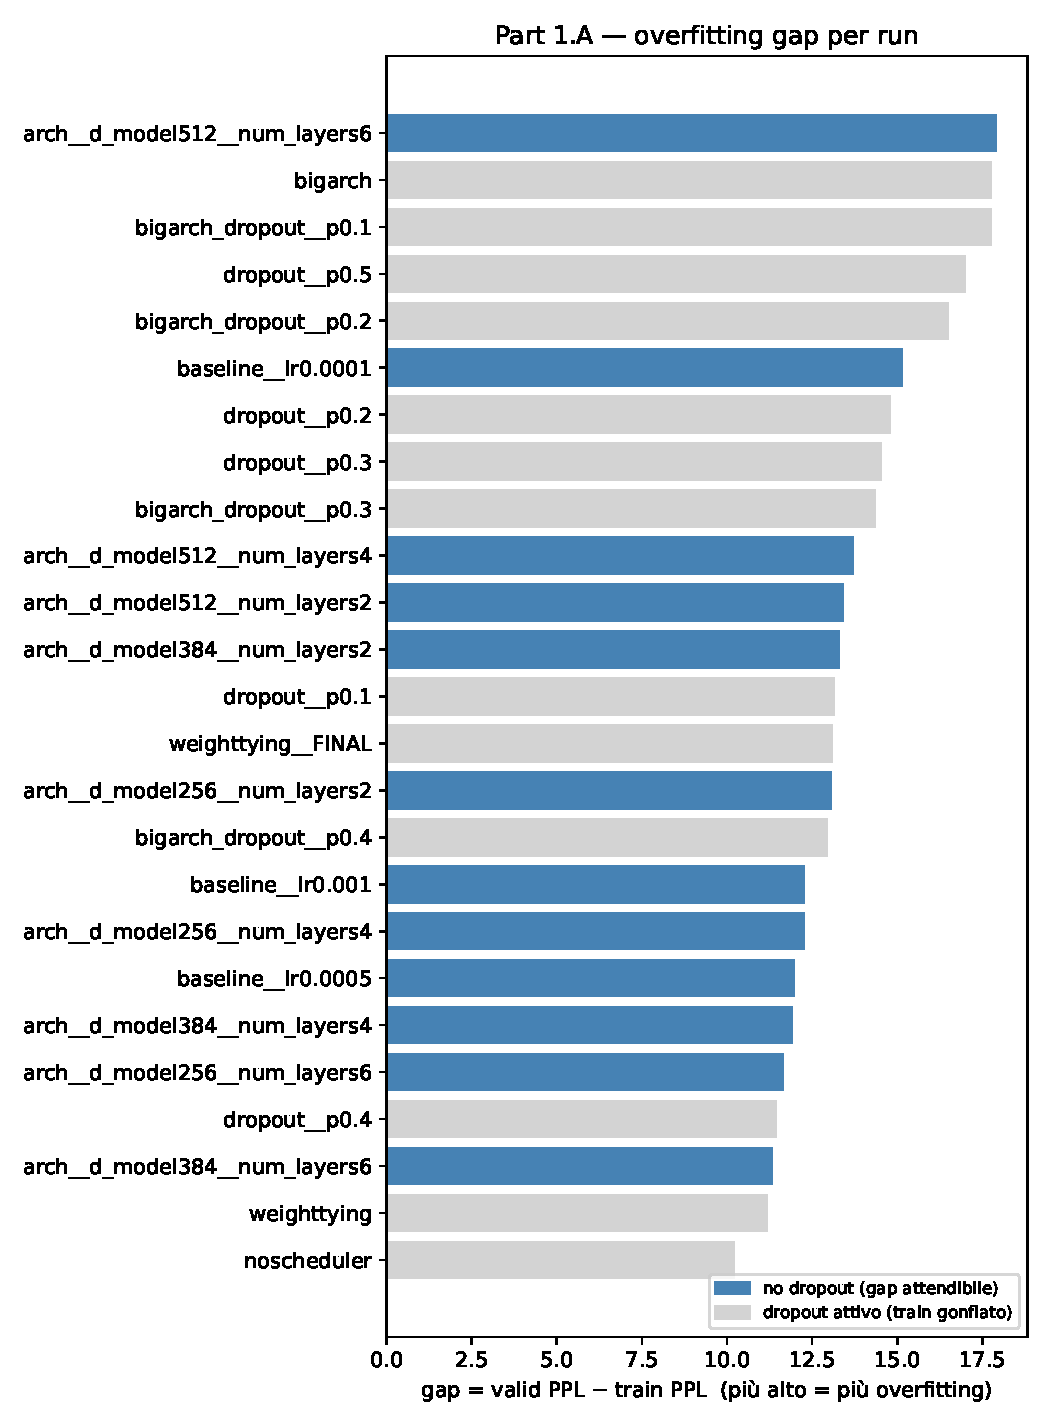
\includegraphics[width=\columnwidth]{figures/overfitting_gaps.pdf}
  \caption{Part 1.A overfitting gap (valid\,$-$\,train PPL) per run. Blue = clean
  no-dropout runs (reliable gap); grey = dropout-active runs (training loss inflated,
  gap not comparable). The clean gaps are sizable ($\approx$11--18) and grow with model
  size: the models overfit, the largest (\texttt{d512/l6}) most.}
  \label{fig:gap}
\end{figure}

\section*{Declaration of AI use}
A generative-AI assistant was used to help structure the experiment pipeline and edit
the language of this report; all architectural choices, experiments and results are the
author's own.

\bibliographystyle{IEEEtran}
\bibliography{mybib}

\end{document}
